\documentclass[12pt, a4paper]{article}
\usepackage[british]{babel}
\usepackage[utf8]{inputenc}
\usepackage{amsmath}
\usepackage{amssymb}
\usepackage{booktabs}
\usepackage{bbold}
\usepackage[hidelinks]{hyperref}
\usepackage{graphicx}

\graphicspath{{img/}}

\title{\textbf{TVD discretization of the Navier-Stokes equations}}
\author{Andrea Vescovini}
\date{\today}

\begin{document}
	\maketitle

\section{The model}
We consider the isothermal Navier-Stokes equations made of a scalar mass 
balance equation \eqref{eq:mass_bal} and a vectorial momentum equation 
\eqref{eq:mom_bal}:
\begin{align}
	\label{eq:mass_bal} \frac{\partial\rho}{\partial t} + \nabla \cdot (\rho 
	\mathbf{v}) = 0&\\
	\label{eq:mom_bal} \frac{\partial{(\rho \mathbf{v}})}{\partial t} + \nabla 
	\cdot (\rho \mathbf{v} \mathbf{v^\mathrm{T}}) - \nabla \cdot \tau + 
	\nabla p = 0&
\end{align}
\begin{itemize}
	\item $\rho$ is the density of the fluid $[kg / m^3]$
	\item $\mathbf{v} = [u, v, w]^\mathrm{T}$ is the velocity vector $[m/s]$
	\item $\tau$ is the viscous stress tensor $[Pa]$
	\item $p$ is the pressure $[Pa]$
\end{itemize}
We consider a Newtonian fluid so that the viscous stress tensor is:
\begin{equation*}
\tau = 2\mu \frac{\nabla \mathbf{v} + \nabla \mathbf{v}^\mathrm{T}}{2} + 
\lambda (\nabla \cdot \mathbf{v}) \mathbb{1},
\end{equation*}
where $\mu$ is the dynamic viscosity and $\lambda$ is a 
dilatation factor. In order to keep a simple model we will consider 
$\lambda = 0$ and neglect $\nabla \mathbf{v}^\mathrm{T}$, so that $\tau = 
\mu \nabla \mathbf{v}$. We have also neglected the gravity vector.
The momentum equation \eqref{eq:mom_bal} becomes:
\begin{equation} \label{eq:mom_bal_simpl}
\frac{\partial{(\rho \mathbf{v}})}{\partial t} + \nabla 
\cdot (\rho \mathbf{v} \mathbf{v^\mathrm{T}}) - \nabla \cdot (\mu \nabla 
\mathbf{v}) + 
\nabla p = 0
\end{equation}

\section{The finite volumes discretization}
We want to discretize the equations 
\eqref{eq:mass_bal},\eqref{eq:mom_bal_simpl} using a finite volume scheme over 
a staggered grid. Moreover we want to employ a second order approximation of 
the convective terms that will be crucial for catching the turbulent eddies in 
a coupled framework.
\begin{figure*}[h]
	\centering
	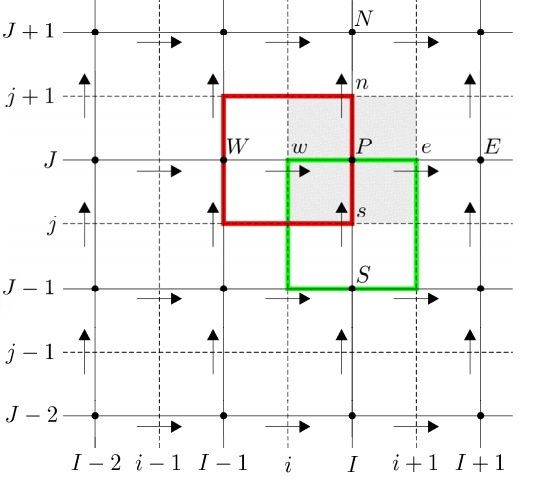
\includegraphics[scale=0.5]{staggered_grid}
	\caption{Control volumes for scalar variables (grey), and for vectorial 
	variables (red and green).}
	\label{fig:grid}
\end{figure*}
In the staggered grid concept we distinguish between the degrees of freedom 
related to scalar variables and those related to vectorial variables. The 
formers are placed at the centre of the cells, as it is for the cell-centred 
schemes, while the components of the vectorial variables are placed at the 
faces of the cells such that they are parallel to the normal vector of the face.

\subsection{The mass balance equation}
For the sake of simplicity we consider now a bi-dimensional domain and 
$\mathbf{v} = [u, v]^{\mathrm{T}}$.
We integrate the mass balance equation \eqref{eq:mass_bal} over the ``grey" 
control 
volume $V = [i,i+~1] \times [j,j+1]$, according to Figure \ref{fig:grid}, and 
we apply the divergence theorem to the convective term:
\begin{equation*}
\int_V \frac{\partial\rho}{\partial t} \; dV + \int_V \nabla \cdot (\rho 
\mathbf{v}) \; dV = \frac{d}{dt} \int_V \rho \; dV + \int_{\partial V} \rho 
\mathbf{v} \cdot \mathbf{n} \; d\sigma = 0
\end{equation*}
$\partial V$ is the boundary of $V$ and in this case $\partial V = e \cap n 
\cap w \cap s$. $\mathbf{n}$ is the outward normal vector to the boundary.
\begin{equation*}
\int_{\partial V} \rho 
\mathbf{v} \cdot \mathbf{n} \; d\sigma = \int_e \rho 
u \; d\sigma + \int_n \rho v \; d\sigma - \int_w \rho u \; d\sigma - \int_s 
\rho v \; d\sigma
\end{equation*}
At this point we have to discretize the equation. For the first term we 
approximate the density with the value at the centre of the control volume:
\begin{equation*}
\frac{d}{dt} \int_V \rho \; dV \simeq \frac{d}{dt} \int_V \rho_{I,J} \; dV = 
\frac{d \rho_{I,J}}{dt} |V|,
\end{equation*}
where $|V|$ denotes the measure of $V$.

For the integrals over the faces we approximate the value of the velocity, i.e. 
the convective field, with the value at the centre of the faces, while for the 
density, i.e. the convected field, we need an extrapolation.
\begin{equation*}
\int_e \rho u \; d\sigma \simeq \int_e \rho_e u_{i+1,J} \; d\sigma = \rho_e 
u_{i+1,J} |e|
\end{equation*}
We would like to approximate $\rho_e$ in order to have a stable scheme of 
second order:
\begin{itemize}
	\item An average between the upwind and the downwind values $\rho_e = 
	(\rho_{I+1,J}+\rho_{I,J})/2$ produces a second 
	order scheme, but not stable because it does not take into account the 
	direction of the flow.
	\item An upwind approximation $\rho_e = \rho^U$ ($\rho_U = \rho_{I,J}$ 
	if $u_{i+1,J}>0$) produces a stable scheme, but of first order and too 
	diffusive.
	\item The QUICK approximation $\rho_e = \frac{3}{8}\rho^D+\frac{6}{8} 
	\rho^U - \frac{1}{8} \rho^{UU}$ produces a scheme of third order, 
	but that may generate unphysical overshoots or undershoots ($\rho^D = 
	\rho_{I+1,J}$ 
	and $\rho^{UU} = \rho_{I-1,J}$ if $u_{i+1,J}>0$).
\end{itemize}
In order to avoid oscillations we would like to have a TVD scheme (total 
variation diminishing) i.e. such that, for a variable $\phi$:
\begin{equation} \label{eq:tvd}
TV(\phi ^{n+1}) \leq TV(\phi^n) \quad \text{for every time-step} \; n,
\end{equation}
where $TV(\phi) = \sum_i |\phi_{i+1} 
- \phi_i|$ is the total variation.\\
According to \cite{sweeby} and \cite{ver_mal} we can achieve this result adding 
to the upwind approximation a second order non-linear correction:
\begin{equation*}
	\rho_e = \rho^U + \frac{1}{2}\psi(r)(\rho^D - \rho^U), \quad r = 
	\frac{\rho^U - \rho^{UU}}{\rho^D - \rho^U}
\end{equation*} 
The function $\psi(r)$ is called \emph{flux limiter} since it limits the second 
order term, ensuring the TVD condition \eqref{eq:tvd}. We have the following 
constraints on this function:
\begin{align*}
\psi(r) = 0 \quad &\text{if} \quad r < 0\\
r \leq \psi(r) \leq \min \{2r, 1\} \quad &\text{if} \quad 0 \leq r \leq 1\\
1 \leq \psi(r) \leq \min \{r, 2\} \quad &\text{if} \quad r > 2
\end{align*}

There are in literature many options for $\psi(r)$, one of the most famous 
is the \emph{min-mod}:
\begin{equation*}
\psi(r) = \max \{0, \min \{ r,1\} \}
\end{equation*}
which adds to the upwind value an increment equal to the smallest 
variation between $\rho^{UU}-\rho^U$ and $\rho^D - \rho^U$. We should also 
point out that when $r < 0$, i.e. when we are in the presence of a local 
extremum, we have only a first-order accuracy.

Coming back to our mass balance equation, we obtain (supposing that $u_{i+1,J} 
>0$, $u_{i,J} > 0$, $v_{I,j+1}>0$, $v_{I,j} >0$):
\begin{multline*}
\frac{d \rho_{I,J}}{dt} |V| + (\rho_{I;J} + \frac{1}{2}\psi(r_e)(\rho_{I+1,J} - 
\rho_{I,J}))u_{i+1,J}|e| +\\
+ (\rho_{I,J} + \frac{1}{2}\psi(r_n)(\rho_{I,J+1} - 
\rho_{I,J}))v_{I,j+1}|n|-\\
	-(\rho_{I-1,J} + \frac{1}{2}\psi(r_w)(\rho_{I,J} - 
	\rho_{I-1,J}))u_{i,J}|w|-\\
	-(\rho_{I,J-1} + \frac{1}{2}\psi(r_s)(\rho_{I,J} - \rho_{I,J-1}))v_{I,j}|s| 
	= 0 \quad \forall {I,J}
\end{multline*}
\subsection{The momentum equation}
For the momentum equation we have different control volumes. Let us integrate 
the equation \eqref{eq:mom_bal_simpl} for the component $u$ over the ``red" 
control volume in Figure \ref{fig:grid}, $\bar{V} = [I-1,I] \times [j,j+1]$:
\begin{multline*}
\int_{\bar{V}} \bigg[ \frac{\partial{(\rho u})}{\partial t} + \nabla 
\cdot (\rho u \mathbf{v} ) - \nabla \cdot (\mu \nabla u) + 
\frac{\partial p}{\partial x} \bigg ]\; dV =\\
=\frac{d}{dt} \int_{\bar{V}} \rho u\; dV+ \int_{\partial \bar{V}} \rho u 
(\mathbf{v} \cdot 
\mathbf{n}) \; d\sigma - \int_{\partial \bar{V}} \mu \frac{\partial u}{\partial 
n} \; d\sigma + \int_{\partial \bar{V}} p n_x \; d\sigma = 0
\end{multline*}
\begin{itemize}
	\item For the storage term we approximate the density with an average:
	\begin{equation*}
\frac{d}{dt} \int_{\bar{V}} \rho u\; dV \simeq \frac{d}{dt} \bigg( 
\frac{\rho_{I,J}+\rho_{I-1,J}}{2} u_{i,J} \bigg)|\bar{V}|
	\end{equation*}
	\item For the convective term we employ again the TVD approximation. We 
	denote by $e,n,w,s$ the four faces of $\partial \bar{V}$, paying attention 
	that they do not correspond to those used before.
	\begin{equation*}
	\int_{\partial \bar{V}} \rho u 
	(\mathbf{v} \cdot 
	\mathbf{n}) \; d\sigma = \int_e \rho u u \; d\sigma + \int_n \rho u v \; 
	d\sigma - \int_w \rho u u \; d\sigma -\int_s \rho u v \; d\sigma
	\end{equation*}
	In the following computations the upwind and downwind values depend on the 
	sign of the transporting field 
	$\mathbf{v}\cdot\mathbf{n}$. 
	\begin{equation*}
	\int_e \rho u u \; d\sigma \simeq 
	\rho_{I,J}\frac{u_{i+1,J}+u_{i,J}}{2}(u^U+\frac{1}{2}\psi(r_e)(u^D-u^U))|e|
	\end{equation*}
	\begin{equation*}
		\int_w \rho u u \; d\sigma \simeq 
		\rho_{I-1,J}\frac{u_{i-1,J}+u_{i,J}}{2}(u^U+\frac{1}{2}\psi(r_w)(u^D-u^U))|w|
	\end{equation*}
	Over the horizontal faces we do not have directly a value for the density, 
	we decide to consider it as a transported quantity so we use the TVD 
	approximation. We split the faces into two sub-faces, for the left one we 
	use the values of the density over the column $I-1$, while for the right 
	one we use the values over the column $I$. Different choices can be 
	probably taken into account. 
	\begin{multline*}
	\int_n \rho u v \; d\sigma \simeq
	\frac{|n|}{2}v_{I,j+1}(\rho^U+\frac{1}{2}\psi(r_n)(\rho^D-\rho^U))
	(u^U+\frac{1}{2}\psi(r_n)(u^D-u^U)) +\\
	+\frac{|n|}{2}v_{I-1,j+1}(\rho^U+\frac{1}{2}\psi(r_n)(\rho^D-\rho^U))
	(u^U+\frac{1}{2}\psi(r_n)(u^D-u^U))
	\end{multline*}
	\begin{multline*}
	\int_s \rho u v \; d\sigma \simeq
	\frac{|s|}{2}v_{I,j}(\rho^U+\frac{1}{2}\psi(r_s)(\rho^D-\rho^U))
	(u^U+\frac{1}{2}\psi(r_s)(u^D-u^U)) +\\
	+\frac{|s|}{2}v_{I-1,j}(\rho^U+\frac{1}{2}\psi(r_s)(\rho^D-\rho^U))
	(u^U+\frac{1}{2}\psi(r_s)(u^D-u^U))
	\end{multline*}
	\item For the diffusive term we employ a standard central finite 
	difference, that is of second order.
	\begin{equation*}
\int_{\partial \bar{V}} \mu \frac{\partial u}{\partial 
	n} \; d\sigma = \int_e \mu \frac{\partial u}{\partial x} \; d\sigma
+ \int_n \mu \frac{\partial u}{\partial y} \; d\sigma
- \int_w \mu \frac{\partial u}{\partial x} \; d\sigma
- \int_s \mu \frac{\partial u}{\partial y} \; d\sigma
	\end{equation*}
	\begin{equation*}
	\int_e \mu \frac{\partial u}{\partial x} \; d\sigma \simeq \mu_{I,J} 
	\frac{u_{i+1,J} - u_{i,J}}{\Delta x} |e|
	\end{equation*}
	\begin{equation*}
	\int_w \mu \frac{\partial u}{\partial x} \; d\sigma \simeq \mu_{I-1,J} 
	\frac{u_{i,J} - u_{i-1,J}}{\Delta x} |w|
	\end{equation*}
	\begin{multline*}
	\int_n \mu \frac{\partial u}{\partial y} \; d\sigma \simeq \frac{|n|}{2} 
	\frac{\mu_{I,J}+\mu_{I,J+1}}{2}\frac{u_{i,J+1}-u_{i,J}}{\Delta y} +\\
+ \frac{|n|}{2} 
\frac{\mu_{I-1,J}+\mu_{I-1,J+1}}{2}\frac{u_{i,J+1}-u_{i,J}}{\Delta 
y}
	\end{multline*}
	\begin{multline*}
	\int_s \mu \frac{\partial u}{\partial y} \; d\sigma \simeq \frac{|s|}{2} 
	\frac{\mu_{I,J}+\mu_{I,J-1}}{2}\frac{u_{i,J}-u_{i,J-1}}{\Delta y} +\\
	+ \frac{|s|}{2} 
	\frac{\mu_{I-1,J}+\mu_{I-1,J-1}}{2}\frac{u_{i,J}-u_{i,J-1}}{\Delta y}
	\end{multline*}
	\item Eventually we have the term with the pressure:
	\begin{equation*}
	\int_{\partial \bar{V}} pn_x \; d\sigma = \int_e p \; d\sigma - \int_w p \; 
	d\sigma \simeq p_{I,J} |e| - p_{I-1,J} |w|
	\end{equation*}
\end{itemize}

The momentum equation for the component $v$ can be discretized in an analogous 
way.

In the implementation the correction terms $\frac{1}{2} \psi(r) (\rho^D - 
\rho^U)$ are treated as \emph{deferred} terms, i.e. we use for them the values 
at the previous Newton iteration.\\
For the time discretization we employ an implicit Euler method.
\begin{thebibliography}{99}\label{sec:bib}
	\bibitem{hirsch} C. Hirsch. \emph{Numerical Computation of Internal and 
	External Flows}, volume 2. Butterworth-Heinemann Limited, 2006.
	
	\bibitem{sweeby} P.K. Sweeby. High Resolution Schemes Using Flux Limiters 
	for Hyperbolyc Conservation Laws. \emph{SIAM J. Numer. Anal.}, 
	21(5):995-1011, 1984.
	
	\bibitem{ver_mal} H.K. Versteeg and W. Malalasekera. \emph{An Introduction 
	to Computational Fluid Dynamics: The Finite Volume Method.} Pearson 
	Education Limited, 2007.
	
\end{thebibliography}
\end{document}